% verisolv — a unified numerical-solver + formal-verification artifact.
% Built for ACM/SIGPLAN venues (POPL Student Research Competition) and the
% Journal of Formalized Reasoning. Compile: latexmk -pdf main.tex
\documentclass[sigplan,nonacm,screen]{acmart}

\settopmatter{printacmref=false}
\setcopyright{none}
\renewcommand\footnotetextcopyrightpermission[1]{}
\pagestyle{plain}

\usepackage{listings}
\usepackage{amsmath}
\usepackage{amssymb}
\usepackage{booktabs}
\usepackage{xcolor}
\usepackage{microtype}
\usepackage{graphicx}
\usepackage{tikz}
\usetikzlibrary{positioning,arrows.meta,fit,backgrounds}

% Soak up the few unavoidable overfull lines caused by long inline code tokens
% (e.g. Lean/Rust identifiers) rather than letting them protrude into the margin.
\setlength{\emergencystretch}{3em}

% ---- Lean / code listing style -------------------------------------------
\definecolor{kw}{RGB}{0,90,160}
\definecolor{cmt}{RGB}{110,120,130}
\definecolor{str}{RGB}{160,60,40}
\lstdefinelanguage{lean}{
  morekeywords={theorem,lemma,def,structure,namespace,end,variable,intro,
    induction,with,calc,have,show,by,exact,fun,forall,Prop,Type,open,import,
    refine,simp,rw,ring,linarith,nlinarith,positivity,push_cast,le_trans},
  sensitive=true,
  morecomment=[l]{--},
  morecomment=[s]{/-}{-/},
  morestring=[b]",
}
\lstdefinelanguage{myrust}{
  morekeywords={fn,let,mut,dyn,impl,struct,enum,pub,use,mod,match,move,return,
    for,in,while,loop,if,else,as,ref,Some,None,Ok,Err,Self,self,where,unsafe},
  sensitive=true,
  morecomment=[l]{//},
  morecomment=[s]{/*}{*/},
  morestring=[b]",
}
\lstset{
  basicstyle=\ttfamily\footnotesize,
  keywordstyle=\color{kw}\bfseries,
  commentstyle=\color{cmt}\itshape,
  stringstyle=\color{str},
  showstringspaces=false,
  breaklines=true,
  breakatwhitespace=false,
  postbreak=\mbox{\textcolor{cmt}{$\hookrightarrow$}\space},
  basewidth={0.5em,0.45em},
  columns=fullflexible,
  frame=single,
  framesep=4pt,
  xleftmargin=4pt,
  inputencoding=utf8,
  extendedchars=true,
  literate=
    {ℝ}{{$\mathbb{R}$}}1 {ℕ}{{$\mathbb{N}$}}1 {≤}{{$\leq$}}1 {≥}{{$\geq$}}1
    {→}{{$\rightarrow$}}1 {∀}{{$\forall$}}1 {∃}{{$\exists$}}1 {₀}{{$_0$}}1
    {₁}{{$_1$}}1 {₂}{{$_2$}}1 {·}{{$\cdot$}}1 {↑}{{$\uparrow$}}1 {ε}{{$\varepsilon$}}1
    {α}{{$\alpha$}}1 {τ}{{$\tau$}}1 {≠}{{$\neq$}}1 {∈}{{$\in$}}1 {⟨}{{$\langle$}}1
    {⟩}{{$\rangle$}}1 {⊢}{{$\vdash$}}1 {λ}{{$\lambda$}}1 {β}{{$\beta$}}1
    {∧}{{$\wedge$}}1 {∨}{{$\vee$}}1 {¬}{{$\neg$}}1 {²}{{$^{2}$}}1
    {ⁿ}{{$^{n}$}}1 {ᵏ}{{$^{k}$}}1,
}

\begin{document}

\title{verisolv: A Unified Artifact Bridging a Numerical ODE/PDE Solver and a
Machine-Checked Convergence Proof}

\author{Anubhav Prasai}
\affiliation{%
  \institution{AIYGO}
  \country{}
}
\email{anubhavprasai123@gmail.com}

\author{Himangsu Adhikari}
\affiliation{%
  \institution{AIYGO}
  \country{}
}
\email{himangsuadk@gmail.com}

\begin{abstract}
Numerical software for differential equations is trusted on the strength of
empirical testing, while the convergence theorems that justify its algorithms
live in textbooks, disconnected from the code that runs. We present
\emph{verisolv}, a single reproducible monorepo that closes part of this gap: a
SciPy-like numerical initial-value and partial-differential-equation
solver whose simplest integrator is accompanied by a machine-checked proof of
convergence. The library exposes a \texttt{solve\_ivp} interface with five ODE
methods (explicit Euler, classical RK4, adaptive Dormand--Prince RK45,
fourth-order Adams--Bashforth, and an implicit backward-differentiation-formula
stiff solver) and two finite-difference PDE solvers (1-D heat and wave),
implemented in Python with an optional Rust kernel exposed through PyO3 that
reproduces the fixed-step RK4 trajectory bit-for-bit and the adaptive RK45
trajectory under an identical step-control law. In parallel, a Lean~4 development
built on Mathlib formalizes the explicit-Euler recurrence \emph{exactly as
implemented} and proves that its global error is $O(h)$ for Lipschitz-continuous
right-hand sides under a standard $O(h^2)$ local-truncation bound, with an
explicit constant $C = C_2\,T\,e^{LT}$. The proof is complete---it contains no
\texttt{sorry} and depends only on Lean's three standard axioms---and the build
itself runs \texttt{\#print axioms} to confirm it. The artifact builds and
validates end to end with four commands (\texttt{pip install}, \texttt{pytest},
\texttt{cargo test}, \texttt{lake build}). We argue that an explicit
\emph{contract} tying the verified recurrence to the executed code is what makes
``implemented and formally verified'' a checkable claim rather than a slogan.
\end{abstract}

\keywords{formal verification, Lean 4, Mathlib, numerical analysis, ordinary
differential equations, Euler method, convergence, Runge--Kutta, PyO3,
reproducibility}

\maketitle

% =========================================================================
\section{Introduction}
\label{sec:intro}

The numerical solution of differential equations is among the most widely
deployed pieces of scientific software, underpinning simulation across physics,
engineering, biology, and finance. The libraries that perform it---SciPy's
\texttt{integrate} module, SUNDIALS, the MATLAB ODE suite---are validated almost
entirely by testing: a method is run on problems with known solutions, and its
observed error is checked against the expected rate. This is necessary but not
sufficient. Testing demonstrates that an implementation \emph{behaves} on the
sampled inputs; it does not establish that the underlying \emph{algorithm} must
converge, nor that the code faithfully realizes the algorithm whose convergence
the textbook proves.

Formal verification offers the missing guarantee, and interactive theorem
provers have matured to the point where the relevant analysis is in reach. The
Lean~4 proof assistant~\cite{demoura2021lean4} and its mathematical library
Mathlib~\cite{mathlib2020} now contain enough real analysis---limits,
derivatives, Grönwall-type inequalities, the exponential function---to state and
prove the convergence of basic numerical schemes. Yet a proof in a vacuum is of
limited engineering value: if the verified recurrence is not demonstrably the
one the production code executes, the proof certifies a different artifact than
the one users run.

This paper presents \textbf{verisolv}, an artifact designed around exactly that
tension. It is a single monorepo containing three cooperating pillars:

\begin{enumerate}
\item a \textbf{Python solver library} with a SciPy-like API, five ODE
integrators, and two PDE solvers, all deterministic and stability-aware;
\item an optional \textbf{Rust numerical kernel} exposed through
PyO3~\cite{pyo3} and built with maturin, accelerating the Runge--Kutta inner
loops while reproducing the fixed-step RK4 trajectory bit-for-bit; and
\item a \textbf{Lean~4 formalization} that proves the explicit Euler method
converges with global error $O(h)$ for Lipschitz right-hand sides.
\end{enumerate}

The contribution is not a new integrator or a new theorem---both the
Dormand--Prince pair~\cite{dormandprince1980} and the convergence of Euler's
method are classical. The contribution is the \emph{bridge}: a deliberate,
auditable correspondence between the recurrence proved correct in Lean and the
recurrence executed in Python, mediated by an explicit interface contract. The
explicit Euler step is kept intentionally trivial---no fused stages, no
adaptivity---precisely so that the Python loop and the Lean definition are
visibly the same object, and neither can drift from the other without violating
the shared contract.

We make the following claims, each backed by an automated check:
\begin{itemize}
\item \textbf{The library is real and correct on its tests.} A \texttt{pytest}
suite of 23 tests checks per-method accuracy, order of convergence, energy
conservation, stiff stability, and agreement with SciPy
(\S\ref{sec:eval}).
\item \textbf{The Rust path is a transparent accelerator.} Compiled RK4
reproduces the Python trajectory to floating-point identity, and the extension
is strictly optional: absent it, the library runs unchanged
(\S\ref{sec:rust}).
\item \textbf{The Euler convergence proof is complete.} It contains no
\texttt{sorry}, and \texttt{\#print axioms} reports dependence only on
\texttt{propext}, \texttt{Classical.choice}, and \texttt{Quot.sound}---Lean's
three standard axioms, with the proof-hole axiom \texttt{sorryAx} absent
(\S\ref{sec:lean}).
\item \textbf{The whole artifact is reproducible.} Four commands build and
validate every pillar from a clean checkout (\S\ref{sec:eval}).
\end{itemize}

% =========================================================================
\section{System Architecture}
\label{sec:arch}

\begin{figure}[t]
\centering
\resizebox{\columnwidth}{!}{%
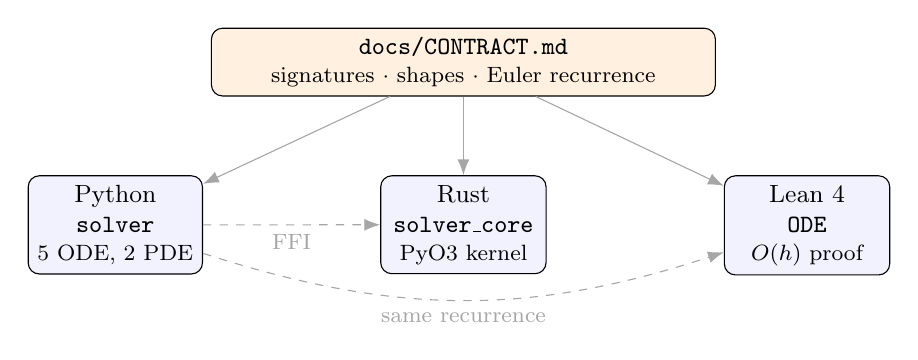
\begin{tikzpicture}[
  font=\small,
  pillar/.style={draw, rounded corners, align=center, minimum height=12mm,
    minimum width=21mm, fill=blue!5},
  contract/.style={draw, rounded corners, align=center, minimum width=64mm,
    minimum height=8mm, fill=orange!12},
  arr/.style={-{Latex[length=2mm]}, gray!70},
]
  \node[contract] (c) {\texttt{docs/CONTRACT.md}\\[-1pt]
    {\footnotesize signatures $\cdot$ shapes $\cdot$ Euler recurrence}};
  \node[pillar, below left=10mm and 1mm of c] (py) {Python\\\texttt{solver}\\[-1pt]
    {\footnotesize 5 ODE, 2 PDE}};
  \node[pillar, below=10mm of c] (rs) {Rust\\\texttt{solver\_core}\\[-1pt]
    {\footnotesize PyO3 kernel}};
  \node[pillar, below right=10mm and 1mm of c] (ln) {Lean 4\\\texttt{ODE}\\[-1pt]
    {\footnotesize $O(h)$ proof}};
  \draw[arr] (c) -- (py); \draw[arr] (c) -- (rs); \draw[arr] (c) -- (ln);
  \draw[arr, dashed] (py) -- node[below, font=\footnotesize]{FFI} (rs);
  \draw[arr, dashed] (py) to[bend right=18]
    node[below=1pt, font=\footnotesize]{same recurrence} (ln);
\end{tikzpicture}%
}
\caption{The three pillars and the contract that binds them. The contract pins
the interfaces and the Euler recurrence; the Python reference, the Rust kernel,
and the Lean proof each conform to it independently. The dashed FFI
(foreign-function-interface) edge marks the Python--Rust boundary.}
\label{fig:arch}
\end{figure}

\subsection{Monorepo layout}
verisolv is organized as a monorepo with one directory per concern
(Figure~\ref{fig:arch}):
\texttt{python\_solver/} (the importable \texttt{solver} package and its tests),
\texttt{rust\_core/} (the \texttt{solver\_core} crate and its maturin packaging),
\texttt{lean/} (the Lean~4 project and its \texttt{ODE} library),
\texttt{benchmarks/} (the SciPy comparison harness), and \texttt{docs/} (the
interface contract and mathematical notes). Keeping the three language
ecosystems in one repository is what lets the artifact tell a single coherent
story while still allowing each pillar to be built and tested in isolation:
\texttt{pytest} runs with no Rust present, \texttt{cargo test} runs with no
Python interpreter, and \texttt{lake build} needs neither.

\subsection{The interface contract}
A plain-text \emph{contract} (\texttt{docs/CONTRACT.md}) is the source of truth
for module boundaries, function signatures, return shapes, and---critically---the
exact form of the Euler recurrence. Because three independent implementations
(Python, Rust, Lean) must agree, the contract pins details that would otherwise
drift: every ODE stepper is a free function returning a canonical
$(t, y, \mathit{info})$ triple with the state array in SciPy
$(n_\text{states}, n_\text{times})$ layout; the adaptive step-control law is
specified constant-for-constant so the Python and Rust RK45 produce identical
trajectories; and the Euler recurrence is fixed as
$y_{k+1} = y_k + h\,f(t_k, y_k)$ with the requirement that the Lean development
match it. The contract is an engineering artifact, not user documentation, and it
is the mechanism by which ``the same recurrence'' is more than a figure of
speech.

\subsection{Dispatch and the failure boundary}
The user-facing driver \texttt{solve\_ivp} is a thin dispatcher: it resolves the
method name, validates the time span and initial state, wraps the user's
right-hand side $f$ in an evaluation counter at the driver boundary (so every
method reports a consistent \texttt{nfev} regardless of internal bookkeeping),
calls the selected stepper, and packages the result. Stepper exceptions are
contained and surfaced as a result object with \texttt{success=False} rather than
propagating, so the public API always returns a well-formed value.

% =========================================================================
\section{The Numerical Solver Library}
\label{sec:lib}

\subsection{ODE integrators}
The library provides five integrators spanning the standard taxonomy.

\paragraph{Explicit Euler} is the first-order scheme
$y_{k+1} = y_k + h\,f(t_k, y_k)$. It is intentionally the simplest stepper and
serves as the \emph{verified anchor}: its loop is line-for-line the recurrence
formalized in Lean (\S\ref{sec:lean}).

\paragraph{Classical RK4} is the fourth-order explicit Runge--Kutta method with
the standard $(1,2,2,1)/6$ weighting. Its global error is $O(h^4)$; halving the
step reduces the error by a factor near $16$, which the test suite checks
directly.

\paragraph{Dormand--Prince RK45} is an embedded $5(4)$ pair~\cite{dormandprince1980}.
Six stages (seven under the first-same-as-last optimization) yield both a
fifth-order solution that advances the state and a fourth-order companion whose
difference estimates the local error. The step is accepted when the
root-mean-square (RMS) scaled
error norm satisfies $\mathrm{err} \le 1$, and the next step is
\[
  h_{\text{new}} = h \cdot \mathrm{clip}\!\left(0.9\,\mathrm{err}^{-1/5},\,0.2,\,5.0\right),
\]
with rejected steps retried at a smaller $h$. The integrator lands exactly on the
final time and reuses the last stage of an accepted step as the first stage of
the next.

\paragraph{Adams--Bashforth 4} is an explicit linear multistep method,
$y_{k+1} = y_k + \tfrac{h}{24}(55 f_k - 59 f_{k-1} + 37 f_{k-2} - 9 f_{k-3})$,
bootstrapped with RK4 for the first three steps. It is fourth-order but uses only
one new right-hand-side evaluation per step.

\paragraph{BDF1/BDF2} is a simplified but genuine implicit stiff solver based on
the backward differentiation formula (BDF). It
bootstraps with backward Euler (BDF1) and continues with BDF2, solving the
implicit system at each step by Newton's method with a forward-difference
Jacobian and an LU solve. Backward Euler is A-stable (indeed L-stable), so the
method stays bounded on stiff problems where explicit schemes would require
prohibitively small steps. Concretely, each step solves the nonlinear residual
$G(z) = z - y_k - h\,f(t_{k+1}, z) = 0$ (for BDF1) by the Newton update
$z \leftarrow z - J^{-1}G(z)$ with $J = I - h\,\partial f/\partial y$ approximated
column-by-column by forward differences. A subtle but real bug surfaced during
testing: seeding Newton with the explicit-Euler predictor $y_k + h f$ diverges on
stiff problems, where $|h\,\partial f/\partial y| \gg 1$ flips the predictor's
sign and the absolute residual at that bad guess can fall under tolerance before
Newton corrects it. Warm-starting from the previous accepted state---sign-correct
and standard for implicit integrators---fixes it, a reminder that the
``simplified'' label hides genuine numerical care.

\subsection{PDE solvers}
Two 1-D finite-difference solvers follow the same ``real, deterministic,
stability-aware'' philosophy, each emitting a Courant--Friedrichs--Lewy (CFL)
warning rather than silently
producing garbage when an explicit scheme's stability criterion is violated.

The \textbf{heat equation} $u_t = \alpha u_{xx}$ offers an explicit
forward-time centered-space (FTCS) scheme, conditionally stable for
$r = \alpha\,\Delta t/\Delta x^2 \le \tfrac12$, and an implicit
Crank--Nicolson scheme that is unconditionally stable and second-order in both
variables, solving a tridiagonal system each step with a sparse direct solver.
The \textbf{wave equation} $u_{tt} = c^2 u_{xx}$ uses explicit leapfrog, stable
under the Courant condition $C = c\,\Delta t/\Delta x \le 1$, with a
second-order Taylor start that injects the initial velocity.

\subsection{Stability analysis}
The stability criteria above are not folklore constants but the output of von
Neumann analysis, which the solvers encode as runtime warnings. Substituting a
Fourier mode $u_j^k = G^k e^{\mathrm{i}\beta x_j}$ into the FTCS update gives the
amplification factor
\[
  G(\beta) = 1 - 4r\sin^2\!\left(\tfrac{\beta \Delta x}{2}\right),
\]
and $|G| \le 1$ for all $\beta$ forces $r \le \tfrac12$. The same substitution into
Crank--Nicolson yields
\[
  G(\beta) = \frac{1 - 2r\sin^2(\beta\Delta x/2)}
                  {1 + 2r\sin^2(\beta\Delta x/2)},
\]
whose magnitude is at most $1$ for \emph{every} $r > 0$, hence unconditional
stability. For leapfrog the amplification factor satisfies a quadratic whose roots
lie on the unit circle exactly when $C \le 1$---the discrete shadow of the
Courant--Friedrichs--Lewy principle that the numerical domain of dependence must
contain the physical one. Each solver computes its mesh ratio, compares it to the
threshold, and emits a typed \texttt{CFLWarning} when the explicit criterion is
violated, so an unstable configuration is reported rather than silently returning
a diverging field. We validate the implicit and explicit schemes against the
analytic fundamental mode $u(x,t) = \sin(\pi x/L)\,e^{-\alpha(\pi/L)^2 t}$ for heat
and the standing wave $u(x,t) = \sin(\pi x/L)\cos(\pi c t/L)$ for the wave
equation.

% =========================================================================
\section{The Rust Kernel and the Foreign-Function-Interface Boundary}
\label{sec:rust}

The performance-critical inner loops of RK4 and RK45 are implemented in Rust in
the \texttt{solver\_core} crate, compiled to a PyO3 extension module and packaged
with maturin as an \texttt{abi3} (stable application binary interface, ABI) wheel---one
binary for CPython~3.10+. The design goal is a \emph{safe} and \emph{testable}
foreign-function-interface (FFI) boundary, achieved by a clean split.

The numerically heavy cores---\texttt{rk4\_core}, \texttt{rk45\_core},
\texttt{bdf1\_core}, and a tridiagonal Thomas solver---take the right-hand side as
a native Rust closure \lstinline[language=myrust]|&mut dyn FnMut(f64, &[f64]) -> Vec<f64>|
and contain \emph{no} PyO3 types. Consequently the crate's unit tests pass a
native Rust closure and run under plain \texttt{cargo test} with no Python
interpreter; 20 such tests cover accuracy, adaptivity, determinism, stiff
stability, and the linear solver.

The only Python-aware code is the thin \lstinline[language=myrust]|#[pyfunction]|
layer, which extracts the initial state, builds the Rust closure from the user's
Python callable (invoked under the global interpreter lock, GIL), and records the
first error or shape
mismatch in an \lstinline[language=myrust]|Option<PyErr>|. On error the closure
returns a zero derivative rather than a NaN, guaranteeing the adaptive loop
terminates promptly; the wrapper then re-raises the recorded error. The Rust
RK45 uses the same step-control law as the Python version, so an accelerated run
reproduces the reference trajectory. For fixed-step RK4 the agreement is exact:
our test suite asserts that the compiled and pure-Python trajectories are
agree to within $10^{-12}$, and in practice the maximum observed difference is
$0$.

On the Python side, the bridge imports \texttt{solver\_core} inside a
\texttt{try/except} that can never raise. Success sets
\texttt{RUST\_AVAILABLE = True} and re-exports the entry points; any failure
(missing wheel, ABI mismatch) sets it to \texttt{False}. The driver consults this
flag when \texttt{use\_rust=True}: if the extension is absent it warns once and
falls back to pure Python. The accelerator is thus entirely optional.

% =========================================================================
\section{Formal Verification of Euler Convergence}
\label{sec:lean}

The Lean development (file \texttt{EulerConvergence.lean}) proves that the
explicit Euler method converges with global error $O(h)$. It is built against
Mathlib pinned to a fixed release, with the toolchain pinned in
\texttt{lean-toolchain} for reproducibility.

\subsection{Setup}
We solve $y'(t) = f(t, y)$ with $y_k \approx y(t_k)$ on the uniform grid
$t_k = t_0 + kh$. All data and hypotheses are bundled in a structure:

\begin{lstlisting}[language=lean]
structure EulerData where
  f : ℝ → ℝ → ℝ
  L : ℝ
  hL : 0 ≤ L
  lipschitz : ∀ t u v : ℝ, |f t u - f t v| ≤ L * |u - v|
  h : ℝ
  hh : 0 < h
  t0 : ℝ
  y0 : ℝ
  Y : ℕ → ℝ                 -- the Euler iterates
  hY0 : Y 0 = y0
  y : ℝ → ℝ                 -- the exact solution
  hinit : y t0 = y0
  C₂ : ℝ
  hC₂ : 0 ≤ C₂
  hYrec : ∀ k, Y (k+1) = Y k + h * f (t0 + k*h) (Y k)
  trunc : ∀ k, |y (t0+(k+1)*h)
      - (y (t0+k*h) + h * f (t0+k*h) (y (t0+k*h)))| ≤ C₂ * h^2
\end{lstlisting}

The field \texttt{hYrec} is the Euler recurrence, identical to the Python loop in
\texttt{methods/euler.py}. We take two analytic facts as \emph{hypotheses}: that
$f$ is Lipschitz in its state argument (\texttt{lipschitz}, constant $L$), and
that the exact solution's one-step truncation residual is bounded by $C_2 h^2$
(\texttt{trunc}). The latter is the standard consequence of a bounded second
derivative ($C_2 = M/2$ with $M = \sup |y''|$); we assume it directly rather than
re-deriving Taylor's theorem, which keeps the development self-contained while the
convergence argument is proved in full.

\subsection{The error recurrence}
Define the global error $e_k = |Y_k - y(t_k)|$. Subtracting the Euler step from
the exact-solution Taylor expansion and applying the triangle inequality and
Lipschitz continuity yields the one-step recurrence, proved completely:

\begin{lstlisting}[language=lean]
theorem error_recurrence (k : ℕ) :
    D.e (k+1) ≤ (1 + D.h * D.L) * D.e k + D.C₂ * D.h^2
\end{lstlisting}

The proof writes the next-step error as a sum of three contributions,
\[
\begin{aligned}
Y_{k+1} - y(t_{k+1}) = {}& \underbrace{(Y_k - y(t_k))}_{A}\\
  &{}+ \underbrace{h\big(f(t_k,Y_k) - f(t_k,y(t_k))\big)}_{B}\\
  &{}+ \underbrace{C_k}_{\text{trunc.}},
\end{aligned}
\]
where $C_k$ is the (negated) local truncation residual. The term $|A|$ is exactly
$e_k$; for $|B|$ we pull out the positive step and apply the Lipschitz hypothesis,
giving $|B| \le hL\,e_k$; and $|C_k| \le C_2 h^2$ is the \texttt{trunc} field.
Mechanizing this is more delicate than the paper mathematics suggests: Lean's
\lstinline[language=lean]|set| tactic folds the abbreviations $A$, $B$, $C_k$,
after which a na\"ive \lstinline[language=lean]|rw| no longer finds the unfolded
pattern, so the bounds must be stated against the folded names and combined with
\lstinline[language=lean]|linarith|. The triangle inequality itself is applied
twice through Mathlib's \lstinline[language=lean]|abs_add_le|.

\subsection{Discrete Grönwall}
The heart of the argument is a self-contained discrete Grönwall inequality:

\begin{lstlisting}[language=lean]
theorem discrete_gronwall {a b : ℝ} {e : ℕ → ℝ}
    (ha : 1 ≤ a) (hb : 0 ≤ b) (he0 : e 0 ≤ 0)
    (hrec : ∀ k, e (k+1) ≤ a * e k + b) :
    ∀ n, e n ≤ b * n * a ^ n
\end{lstlisting}

It is proved by induction on $n$. We deliberately use the
polynomial-times-exponential form $e_n \le b\,n\,a^n$ rather than the geometric
quotient $b(a^n - 1)/(a-1)$: the former needs no division and no $a \ne 1$ side
condition, yet is exactly strong enough for the $O(h)$ result. The base case is
$e_0 \le 0 = b\cdot 0\cdot a^0$. For the step, from
$e_{k+1} \le a\,e_k + b$ and the inductive hypothesis $e_k \le b\,k\,a^k$ we obtain
$a\,e_k \le a\cdot b\,k\,a^k = b\,k\,a^{k+1}$, and since $a \ge 1$ implies
$a^{k+1}\ge 1$ and $b \ge 0$ we have $b \le b\,a^{k+1}$; adding gives
$e_{k+1} \le b\,k\,a^{k+1} + b\,a^{k+1} = b\,(k+1)\,a^{k+1}$. The lone subtlety in
Lean is that the natural-number cast of $k+1$ must be normalized with
\lstinline[language=lean]|push_cast| before \lstinline[language=lean]|ring| closes
the arithmetic, since $\uparrow(k+1)$ and $\uparrow k + 1$ are equal but not
definitionally so. We also prove $1 \le a^m$ inline rather than depend on a
particular library lemma name, a small hedge against version drift
(\S\ref{sec:eval}).

\subsection{The convergence theorem}
Combining the two lemmas with $a = 1 + hL$, $b = C_2 h^2$, the bound
$(1+hL)^n \le e^{nhL} \le e^{LT}$ for $nh \le T$, and $b\,n \le C_2 T h$ gives the
main result:

\begin{lstlisting}[language=lean]
theorem euler_global_error_le (T : ℝ) (hT : 0 ≤ T) :
    ∃ C : ℝ, 0 ≤ C ∧
      ∀ n : ℕ, (n : ℝ) * D.h ≤ T →
        |D.Y n - D.y (D.t n)| ≤ C * D.h
\end{lstlisting}

The witness is the \emph{explicit} constant $C = C_2\,T\,e^{LT}$. Because $C$ is
independent of $h$, halving the step halves the guaranteed error bound: the method
is first-order convergent.

\subsection{Trusting the proof}
A proof is only as trustworthy as its dependencies. We verify two things. First,
the source contains no \texttt{sorry} or \texttt{admit}. Second, and more
strongly, \texttt{\#print axioms} on the main theorem reports
\[
  \texttt{[propext, Classical.choice, Quot.sound]},
\]
the three standard axioms underlying Mathlib. The proof-hole axiom
\texttt{sorryAx} is \emph{absent}, which is a machine-checked guarantee that no
gap was tactically hidden anywhere in the dependency graph. The same holds for
\texttt{discrete\_gronwall} and \texttt{error\_recurrence}.

% =========================================================================
\section{The Bridge}
\label{sec:bridge}

The project's central idea is that the \emph{same} recurrence is implemented and
verified. The correspondence is concrete and maintained on three levels.

\begin{table}[t]
\caption{The correspondence between executed code and proof.}
\label{tab:bridge}
\small
\resizebox{\columnwidth}{!}{%
\begin{tabular}{@{}ll@{}}
\toprule
\textbf{Lean (\texttt{EulerConvergence.lean})} & \textbf{Python (\texttt{euler.py})}\\
\midrule
\texttt{Y}, \texttt{hYrec} & the \texttt{y += h*f(t,y)} loop\\
\texttt{t k = t0 + k*h} & the uniform time grid\\
\texttt{L}, \texttt{lipschitz} & well-posedness of $f$\\
\texttt{euler\_global\_error\_le} & first-order rate the tests observe\\
\bottomrule
\end{tabular}%
}
\end{table}

First, the recurrences are textually identical (Table~\ref{tab:bridge}); the
Python module and the Lean file cross-reference each other by path. The Python
inner loop reads
\begin{lstlisting}[language=Python]
# Lean recurrence: y_{k+1} = y_k + h f(t_k, y_k)
for k in range(n_steps):
    yk = yk + h_eff * f(tk, yk)
    tk = t0 + (k + 1) * h_eff
\end{lstlisting}
and the Lean field \texttt{hYrec} states
\lstinline[language=lean]|Y (k+1) = Y k + h * f (t0 + k*h) (Y k)|---the same
object, modulo the grid-time abbreviation $t_k = t_0 + kh$ that both sides share.

Second, the contract (\S\ref{sec:arch}) pins the recurrence, so neither side can
change without an auditable edit to the shared specification. Third, the empirical
and the formal meet in the evaluation: the test suite \emph{observes} first-order
accuracy on $y' = -y$ (with $f$ Lipschitz, $L=1$), the exact rate the theorem
\emph{guarantees}. We are explicit about scope: only Euler is formally verified.
The higher-order methods are validated numerically. Euler is the verified anchor;
the rest is empirical evidence built outward from it.

% =========================================================================
\section{Evaluation}
\label{sec:eval}

\subsection{Reproducibility}
From a clean checkout the artifact builds and validates with four commands:
\texttt{pip install -e .} (the Python package), \texttt{pytest} (the test suite),
\texttt{cargo test} (the Rust kernels), and
\texttt{lake exe cache get \&\& lake build} (the proof). An optional fifth step,
\texttt{maturin develop --release} followed by a second \texttt{pytest} run,
builds the Rust extension and activates the accelerated-path cross-checks. All
toolchain versions are pinned. The test suite reports 23 passing tests; with the
Rust extension built, the previously skipped cross-checks activate and confirm
Rust/Python parity. The Rust crate reports 20 passing unit tests. The Lean
library builds cleanly, and \texttt{\#print axioms}---run as part of
\texttt{lake build}---confirms the proof depends only on the three standard
axioms with \texttt{sorryAx} absent.

\subsection{Numerical accuracy versus SciPy}
Table~\ref{tab:bench} reports our solvers against SciPy's
\texttt{solve\_ivp} on four problems, measuring maximum error
against an analytic or high-accuracy reference. On exponential decay our adaptive
RK45 reaches $8.7\times10^{-8}$ at $248$ right-hand-side evaluations, matching
SciPy's $9.9\times10^{-8}$ at the same evaluation count---unsurprising, as both
implement the same Dormand--Prince pair. On the harmonic oscillator and
Lotka--Volterra the agreement is similarly close. On the stiff Robertson kinetics
our fixed-step BDF reaches comparable accuracy to SciPy's adaptive
variable-order BDF, though over an order of magnitude slower and at roughly
$60\times$ the right-hand-side evaluations---an expected consequence of fixed
stepping, and a natural target for future adaptivity.

\begin{table}[t]
\caption{Maximum error, wall-clock time, and right-hand-side evaluations versus
SciPy. ``ours'' denotes the verisolv solver; time is the minimum over repeated
runs. Lower is better throughout.}
\label{tab:bench}
\small
\resizebox{\columnwidth}{!}{%
\begin{tabular}{@{}llrrr@{}}
\toprule
Problem & Method & Max error & Time (s) & \texttt{nfev}\\
\midrule
exp.\ decay      & RK45 (ours)  & $8.70\times10^{-8}$ & $0.010$ & 248\\
exp.\ decay      & RK45 (scipy) & $9.93\times10^{-8}$ & $0.005$ & 248\\
harmonic         & RK45 (ours)  & $2.49\times10^{-6}$ & $0.025$ & 728\\
harmonic         & RK45 (scipy) & $2.50\times10^{-6}$ & $0.018$ & 716\\
Lotka--Volterra  & RK45 (ours)  & $4.02\times10^{-4}$ & $0.054$ & 1400\\
Lotka--Volterra  & RK45 (scipy) & $3.89\times10^{-4}$ & $0.045$ & 1394\\
Robertson (stiff)& BDF (ours)   & $1.65\times10^{-6}$ & $1.56$  & 20058\\
Robertson (stiff)& BDF (scipy)  & $6.87\times10^{-7}$ & $0.066$ & 329\\
\bottomrule
\end{tabular}%
}
\end{table}

\subsection{The verified rate, observed}
\begin{figure}[t]
\centering
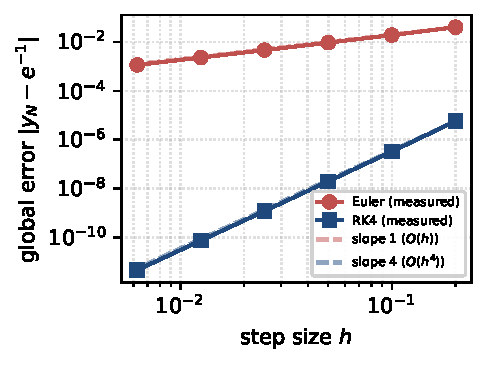
\includegraphics[width=0.82\columnwidth]{convergence.pdf}
\caption{Global error versus step size for explicit Euler and RK4 on
$y'=-y$, log--log axes, with reference slopes. A least-squares fit gives empirical
orders $1.02$ (Euler) and $4.04$ (RK4). The measured Euler slope of $1$ is the
numerical realization of the $O(h)$ rate proved by
\texttt{euler\_global\_error\_le}.}
\label{fig:convergence}
\end{figure}
The test suite checks that explicit Euler on $y'=-y$ exhibits genuine first-order
behavior---accurate to a loose tolerance but not accidentally exact---and that
RK4 exhibits its fourth-order rate, with the error ratio between step sizes
$h=0.1$ and $h=0.05$ falling in $[12,20]$ (the theoretical value is $16$).
Figure~\ref{fig:convergence} makes the rates visible across a sweep of step sizes:
a least-squares fit on the log--log data recovers empirical orders of $1.02$ for
Euler and $4.04$ for RK4. The first-order Euler observation is the numerical
shadow of \texttt{euler\_global\_error\_le}---the theorem and the measurement
agree.

\subsection{Test-suite coverage}
The 23 \texttt{pytest} cases are not smoke tests but targeted checks of numerical
properties. For ODEs they verify: per-method accuracy on exponential decay (Euler
loose but genuinely first order, RK4/RK45 to $10^{-6}$); the harmonic oscillator
against $\cos$/$-\sin$ with energy conservation over a full period; Lotka--Volterra
positivity and oscillation together with an endpoint cross-check of our RK45
against SciPy's to $10^{-4}$; bitwise determinism of repeated calls; the RK4
order-of-convergence ratio; AB4 and BDF accuracy on decay; and BDF stability on a
stiff linear problem. When the Rust extension is present, two further cases assert
Rust/Python RK4 identity and a version probe. For PDEs the suite checks
Crank--Nicolson against the analytic heat mode, the FTCS CFL warning firing
exactly when $r>\tfrac12$, the FTCS stable regime, the leapfrog standing wave, and
the wave Courant warning. The 20 Rust unit tests independently cover the kernels,
the adaptive controller, the Thomas solver, and the stiff path.

\subsection{Reproducibility as an engineering discipline}
Pinning the proof to a fixed Mathlib release is not a formality. Mathlib evolves
rapidly, and lemma names drift between versions: in bringing the development up on
the pinned toolchain we encountered exactly this, with the triangle inequality
formerly spelled \lstinline[language=lean]|abs_add| now requiring
\lstinline[language=lean]|abs_add_le| and the power-monotonicity lemma
\lstinline[language=lean]|pow_le_pow_left| renamed to
\lstinline[language=lean]|pow_le_pow_left₀|. A proof script that built last year
may simply fail to elaborate today. We therefore pin both the Lean toolchain
(\texttt{lean-toolchain}) and the exact Mathlib revision, and the build step uses
\texttt{lake exe cache get} to fetch Mathlib's prebuilt object files---without it,
a from-source Mathlib compilation dominates build time by orders of magnitude. A
second lesson concerns robustness: where possible we replaced automation that
silently depends on the ambient hypothesis set (for instance
\lstinline[language=lean]|positivity|, which could not see a structure field's
nonnegativity proof) with explicit lemma applications such as
\lstinline[language=lean]|mul_nonneg|, trading brevity for stability against
library evolution. These choices are why the artifact's four-command validation
remains reproducible rather than aspirational.

% =========================================================================
\section{Related Work}
\label{sec:related}

\paragraph{Verified numerics.}
Formal verification of numerical analysis has a substantial history in
higher-order logic. Immler and Hölzl verified ODE flows and a Runge--Kutta
method in Isabelle/HOL, including rigorous enclosures of
solutions~\cite{immler2012}; Immler's later work produced a \emph{verified,
executable} ODE solver with rigorous Runge--Kutta integration, obtained by
Isabelle code extraction and applied to the Lorenz attractor~\cite{immler2018}.
That line of work is the closest prior art to our pitch: it achieves a
verified-to-executable path via extraction with rigorous enclosures, whereas
verisolv deliberately keeps the verified core minimal and bridges it to
independently written multi-language code by an explicit contract---a lighter,
more replicable correspondence at the cost of the extraction guarantee.
Boldo and collaborators verified a C program implementing a finite-difference
scheme for the wave equation, bounding both the method and round-off
error~\cite{boldo2013wave}. The CompCert verified C compiler~\cite{leroy2009},
with its Flocq-based IEEE-754 semantics, shows that the compilation and
floating-point layers can themselves be verified---complementary to the
algorithm-level guarantee we provide, and a route toward closing the
real-versus-float gap we leave open (\S\ref{sec:future}). Our aim is
narrower and more pedagogical: a tight, finishable Euler convergence proof in
Lean~4/Mathlib, deliberately wired to a running multi-language library.

\paragraph{Lean and Mathlib.}
Lean~4~\cite{demoura2021lean4} and Mathlib~\cite{mathlib2020} provide the real
analysis our proof rests on. Mathlib already contains Grönwall-type inequalities
and the Picard--Lindelöf theorem for ODE existence and uniqueness; we use the
elementary parts and prove a self-contained discrete Grönwall bound tailored to
the Euler recurrence. We are clear-eyed about the formalization's standing: its
novelty is not new analysis---the discrete Grönwall induction and error
recurrence are elementary by Mathlib's standards---but the \emph{code-tied
packaging}, the fact that the verified recurrence is the one a running solver
executes. For a formalization-focused reading, the natural way to deepen the Lean
content is to discharge the local-truncation hypothesis from a bound on $y''$
using Mathlib's Taylor-theorem infrastructure, which we leave to future work
(\S\ref{sec:future}).

\paragraph{Numerical libraries.}
SciPy's \texttt{solve\_ivp}~\cite{scipy2020} is the reference API our design
echoes. The Rust acceleration via PyO3~\cite{pyo3} follows the now-common pattern
of a Python front-end over a compiled kernel.

% =========================================================================
\section{Discussion and Future Work}
\label{sec:future}

verisolv is deliberately scoped: the verified core is Euler, and the truncation
bound is a hypothesis rather than a theorem derived from a bound on $y''$. The
clearest next step is to discharge that hypothesis inside Lean using Mathlib's
Taylor-theorem infrastructure, removing the last analytic assumption. Beyond
that, the same contract-driven methodology extends to verifying the order of RK4
or the A-stability of backward Euler, and to connecting the discrete PDE schemes
to their continuous stability analyses. A more ambitious direction is to narrow
the implementation gap further---for instance by extracting executable Lean or by
generating the Python and Rust Euler loops from the verified definition, so that
the correspondence is mechanical rather than maintained by contract.

\paragraph{Threats to validity}
We are candid about what the artifact does and does not establish. The proof
certifies the \emph{algorithm}---the abstract Euler recurrence over the reals---not
the floating-point Python code that approximates it; rounding error is outside the
model, as is the equivalence between the real-number recurrence and its IEEE-754
realization. The correspondence between the Lean recurrence and the executed loop
is maintained \emph{socially}, by the contract and by cross-referencing comments,
not mechanically; a sufficiently careless edit could desynchronize them without
tripping a build failure, which is precisely why we regard mechanical generation
as the most valuable future direction. The Lipschitz and truncation facts are
assumed rather than derived. Finally, the higher-order and PDE methods carry no
formal guarantee at all---their evidence is empirical. None of these caveats
undercut the central claim, which is narrow by design: that a specific, classical
convergence result can be proved with no holes and tied, auditably, to running
code.

% =========================================================================
\section{Conclusion}
\label{sec:conclusion}

We presented verisolv, a single reproducible artifact in which a SciPy-like
numerical solver and a machine-checked convergence proof share one narrative. The
library provides five ODE integrators and two PDE solvers with an optional Rust
kernel that reproduces the fixed-step RK4 trajectory exactly; the Lean development
proves explicit Euler converges at $O(h)$ with an explicit constant and no proof
holes, certified by \texttt{\#print axioms}. The connective tissue is an explicit
contract that keeps the verified recurrence and the executed code provably in
step. We believe this contract-driven bridge---rather than either pillar
alone---is the reusable idea: it turns ``implemented and formally verified'' from
a claim into something a reader can check with four commands.

\section*{Artifact Availability}
The complete artifact---Python package, Rust crate, Lean proof, benchmarks, and
documentation---builds and validates with the four commands of
\S\ref{sec:eval}. Toolchain versions are pinned for reproducibility.

\bibliographystyle{ACM-Reference-Format}
\bibliography{refs}

\appendix
\section{The Discrete Grönwall Proof in Full}
\label{app:gronwall}
For concreteness we reproduce the complete, \texttt{sorry}-free Lean source of the
discrete Grönwall lemma (\S\ref{sec:lean}), the inductive heart of the convergence
argument. It depends only on Mathlib's three standard axioms.

\begin{lstlisting}[language=lean]
theorem discrete_gronwall {a b : ℝ} {e : ℕ → ℝ}
    (ha : 1 ≤ a) (hb : 0 ≤ b) (he0 : e 0 ≤ 0)
    (hrec : ∀ k, e (k + 1) ≤ a * e k + b) :
    ∀ n, e n ≤ b * n * a ^ n := by
  have ha0 : 0 ≤ a := le_trans zero_le_one ha
  -- 1 ≤ aⁿ, proved inline to avoid a library name.
  have hpow_ge_one : ∀ m : ℕ, (1 : ℝ) ≤ a ^ m := by
    intro m
    induction m with
    | zero => simp
    | succ k ih => rw [pow_succ]; nlinarith [ih, ha]
  intro n
  induction n with
  | zero => simpa using he0
  | succ k ih =>
    push_cast
    have hstep : e (k + 1) ≤ a * e k + b := hrec k
    have hmul : a * e k ≤ a * (b * k * a ^ k) :=
      mul_le_mul_of_nonneg_left ih ha0
    have hb_le : b ≤ b * a ^ (k + 1) := by
      nlinarith [hpow_ge_one (k + 1), hb]
    calc
      e (k + 1) ≤ a * e k + b := hstep
      _ ≤ a * (b * k * a ^ k) + b := by linarith
      _ = b * k * a ^ (k + 1) + b := by rw [pow_succ]; ring
      _ ≤ b * k * a ^ (k + 1)
            + b * a ^ (k + 1) := by linarith
      _ = b * ((k : ℝ) + 1) * a ^ (k + 1) := by ring
\end{lstlisting}

The convergence theorem instantiates this with $a = 1 + hL$ and $b = C_2 h^2$,
bounds $(1+hL)^n \le e^{LT}$ via Mathlib's \lstinline[language=lean]|Real.add_one_le_exp|
together with \lstinline[language=lean]|pow_le_pow_left₀|, and discharges the final
nonnegativity obligations with explicit \lstinline[language=lean]|mul_nonneg|
applications rather than \lstinline[language=lean]|positivity|, for the
robustness reasons discussed in \S\ref{sec:eval}.

\end{document}
